\documentclass{llncs}
% If the IEEEtran.cls has not been installed into the LaTeX system files, 
% manually specify the path to it: e.g.,
% \documentclass[conference]{../sty/IEEEtran} 

\usepackage{graphicx,times,amsmath} % Add all your packages here
\usepackage{url}
\usepackage{subfigure}

\begin{document}
% Máximo 6 páginas. No lo toques con xemacs

% paper title: Must keep \ \\ \LARGE\bf in it to leave enough margin.
\title{Revisiting volunteer browser-based computing}

\author{V.M. Rivas \inst{1} \and J.J. Merelo \inst{2}}
\institute{ U. Ja\'en (Spain)
\and
U. Granada (Spain)}
% \author{Juan Juli\'an Merelo-Guerv\'os, Pedro A. Castillo, JLJ Laredo,
% A. Mora García}
% % avoiding spaces at the end of the author lines is not a problem with
% % conference papers because we don't use \thanks or \IEEEmembership
% % use only for invited papers
% %\specialpapernotice{(Invited Paper)}
% \institute{Departamento de Arquitectura y 
% Tecnología de Computadores\\
% ETS Ingeniería Informática y Telecomunicaciones\\
% University of Granada (Spain)\\
% email: {\sf jj@merelo.net}}
% make the title area
\maketitle

\begin{abstract}
In this paper we present a new distributed
 evolutionary computation system that uses the computational capabilities of the
 web browser. Using 
Asynchronous JavaScript and JSON (JavaScript Object Notation, a
 serialization protocol) allows anybody with a web browser to participate in experiments with little effort, or none at all. Since, in
this case, computing becomes a social activity and is inherently
impredictable, in this
 paper we will explore the performance of this kind of virtual
 computer by solving simple problems such as the
 Royal Road function and an equation and analyzing how many machines and evaluations
it yields. We will also examine possible performance bottlenecks
 and how to solve them, and, finally, issue some advice on how to set
 up this kind of experiments to maximize turnout and, thus,
 performance. This paper attempts to reproduce results of older papers
 using modern browsers and all kind of devices that, nowadays, hava
 JavaScript integrated in the browser, and is a complete rewrite of
 the code using the popular MOOTools library. % \cite{mootools}. % sólo se menciona aquí...
% Algo sobre los resultados
\end{abstract}

% no key words

\section{Introduction and state of the art}
\label{sec:intro}
% no \PARstart
Application--level networks (ALNs), are configured as a set of
clients/servers ({\em servents}) that
can provide their spare CPU cycles by means of a downloadable
application, establishing a distributed computation network which can
provide ad hoc computational power. Some ALNs
like SETI@Home have been quite successful \cite{david-seti:home},
creating a virtual computer that has proccesed a good amount of
teraflops, while other 
experiments such as Popular Power (and most others, in fact) have not\cite{DBLP:conf/p2p/2005lncs}. 

The key feature of these application--level networks is the simplicity
of use: we believe that the best way to obtain the participation of as
many users as possible is to make it as very simple. In particular, it
will be easier if they do not need to download a special application
(such as a screen-saver) to participate, as is needed in BOINC, the
sucessor to SETI@Home. For this reason, we are exploring the use of
applications that are commonly installed in the user's computer, such
as the web browser, which is available even in PDAs and some cellular
phones\footnote{Whose computing power are similar to four-year-old
desktop machines}.  Moreover, most browsers natively include a
JavaScript
interpreter~\cite{js:reference} or
virtual machine. JavaScript is an interpreted language\footnote{which
has nothing to do with Java, other than the name and its C inherited syntax},
initially proposed by Netscape, and later adopted as an
ECMA standard \cite{ECMA-262}.  In this
way, most browsers are compatible, at least at a language level (not
always at the level of browser objects, where there exists a
reasonable compatibility, anyway). Most browser also include elements
such as a Java virtual machine and a Flash plugin, which, with
ActionScript, has more or less the same capabilities. However, there
are several disadvantages to these: they might or might not be present
(they are not {\em native}), they are {\em noisy} in the sense that,
since they act as plugins, their execution can be noted by the
user, their programs are more heavyweight than simple text code, and,
finally, its integration with the browser is more awkward than the
seamless integration that JavaScript offers. In any case, most things
said here for JavaScript also apply to these and other plugins.

By itself, an interpreted languaje is not enough for creating a
metacomputer if there is no way to convey information back from the
client to the server in a seamless way. The ability to use the virtual
machine included in browsers for distributed computing appeared with
the {\sf XmlHttpRequest} object, which allows asynchronous petitions to the
server, in what has been called AJAX, Asynchronous JavaScript and
XML~\cite{wiki:AJAX}. AJAX is just one of the possible ways to
perform asynchronous client-server communication, the others being
AJAJ (Asynchronous JavaScript and JSON), and {\em remoting} using
applets or embedded objects. However, it is quite popular, and a wide
user base and documentation is available for it, using any of these
asynchronous client/server communication protocols. The traditional client/server model becomes then
more egalitarian, or closer to a peer to peer model, since a
bidirectional communication line appears: the browser can make calls to the
server, do some computation and later send the results to the server.

AJAX (and AJAJ, which differ only in the way the communication is
serialized) works as follows: the {\sf XmlHttpRequest} is provided 
with a request to the server and a pointer to a {\em callback} function. 
The request generates an event, which is asynchronously activated when a
reply is received  making use of the
 {\em callback} function. 
Following this approach the browser is not locked, providing a way to
program applications that are similar to  the ones used at the
desktop, in the sense that they do not have to wait for the
application response to be loaded
and rendered on the screen every time a request is made. It also means
that a the user clicking on the {\sf Submit} button is no longer
needed to initiate communication with the server; any JavaScript
thread can do so, with the constraint that the only server they can
communicate with is the one that hosts the page the script is included
in. On the other side, this provides a way to use the browser for application
level networks that create distributed computing systems,
since the request-response loop does not need the user participation in a
fashion very similar  to any other distributed computing application;
these ALN can be controlled from the server with any programming
language. Of course, it can also be combined with other distributed
programming frameworks based on OpenGrid~\cite{ogsa} or other
distributed computing paradigms. % esto es más bien viejo, habría que
                                % actualizarlo con nubes y cosas así y
                                % últimos trabajos nuestros


This paper presents performance measurements on the jsEO ({\em
  JavaScript Evolving Objects}, pronounce it yi-see-oh) system, which uses PHP 
 (on the server) and JavaScript on the client. The genetic algorithm is carried out  on the clients,
with the server used  for interchange of information among
them. We will perform several experimentes in which clients donate
computing power by just loading a web page to find out what kind of
performance we can expect from this kind of setup, from the number of
machines available to the number of evaluations each one of them
usually performs; as we will show, this kind of setup is ready to take more
computing-intensive experiments without the need of an expensive server or cluster
setup. 

Evolutionary computation is quite adequate for this
kind of distributed environment for several reasons: it is a population based method,
so computation can be distributed among nodes (via distribution of
population) in many different ways;
besides, some works suggest that there are synergies among evolutionary
algorithms and parallelization: isolated populations that are
connected only eventually avoid the loss of diversity and produce
better solutions in fewer time obtaining, in some cases, superlinear
accelerations~\cite{cantu-paz:migration-policies}. Of course, with a suitable work division method, many other algorithms
could be adapted to browser-based distributed computation; however, in
this paper will solve only genetic algorithms, and concentrate on raw
performance, rather than algorithmic behavior. 

Browser based computation falls within the ream of the so called  {\em volunteer
computing}~\cite{sarmenta-bayanihan,hpvc} systems are
application-level networks set up so that different people
can donate resources for a joint computing  effort.
The best known project is SETI@home\footnote{See
\url{http://setiathome.berkeley.edu/} for downloading the software  and some
reports.}, which, from the user's point of view, is a screen-saver which has to be
downloaded and installed; when the user's CPU is not busy it performs
several signal analysis operations.
Some companies related to volunteer computing, such as Popular Power (and
others; they are referenced,
for example, in~\cite{Cappello}) did some experimentation with Java based
clients, but none has had commercial success; on the other hand, the
SETI@Home program has been open-sourced and extended as the BOINC
(Berkeley Open Infrastructure for Network Computing) 
framework \cite{boinc_grid04}. This kind of volunteer computing has
been adapted to evolutionary computation in several occasions, using
frameworks such as DREAM \cite{LNCS2439:ID197:pp665}, which includes a
Java-based virtual machine, GOLEM@Home and G2-P2P \cite{G2-P2P}. Both approaches
acknowledge that to achieve massive scalability, a peer to peer (P2P)
approach is advisable, since it eliminates bottlenecks and single
points of failure. 

There are mainly two problems in this kind of networks: first of all,
it is important not to abuse volunteers CPU resources; secondly, a
sufficient number of users is needed in order to be able to do the
required computation, which can be a problem on its own if there are
too many of them, bringing the network, or at least the
solution-collecting node, to its knees. A third problem is that
performance prediction is difficult when neither the number of
participants nor their individual node performances are known in
advance.

In any case, we believe that the best way to obtain a good amount of
users is to make it easy for them to participate, using technologies
available in their computers, as the browser is. In fact, some
suggestions were published (for example, the one of Jim Culbert in his
weblog \cite{ajax:dc}, and in some mailing lists), and, besides our
own \cite{gecco07:workshop:dcor}, there have been some recent papers
and reports on similar setups. For instance, W. Langdon has been
running for some time an interactive evolution experiment using
JavaScript in the browser \cite{langdon:2005:metas}, which was mainly
intended for achieving high diversity in a fractal snowflake design
than high performance. Even more recently, Klein and Spector
\cite{unwitting-ec} present a system based on the Push3 language,
which is compiled to JavaScript in the browser. This system would be
the closest to what we are presenting in this paper. 

The proposed approach could also be considered as {\em parasitic
computing} since, as stated in Section~\ref{sec:intro}, the only
participation from the user will be to load a web page and click on a
button; in fact, any AJAX-based could use these resources without his
acquiescence (and, in any case, it would be desirable to run without
causing much trouble).  The concept was introduced by Barab\'asi
in~\cite{Barabasi2001Parasitic}, and followed by others (for instance,
Kohring in \cite{kohring-2003-14}).  In that work they proposed to use
the Internet routers to compute a {\em checksum} by means of a set of
specially crafted packets, whose aggregated result would be used to
solve the SAT problem. Anyway, although the concept is interesting,
there seems not to be a continuation for this work (at least openly),
probably due to its inherent dangers (as analyzed in a paper by Lam et
al.  \cite{puppetnets}).

The virtual machine embedded into the browser provides a way to easily
do that kind of  sneaky/parasitic computing, but JavaScript faces the
handicap of being an interpreted language, which means that the efficiency of different
implementations varies wildly. Moreover, it is not optimized for
numerical computation but for object tree 
management (the so called DOM, document
object model) and strings.
Nevertheless its wide availability makes us think about considering it, at
least as a possibility to be explored.

The rest of the paper is organized as follows: experimental setup is described next,  experiments and results are shown in section 
\ref{sec:exp} and discussed in \ref{sec:conc}, along with future lines
of work. 

\section{The jsEO library}
\label{sec:jseo}
In order to provide a modular, flexible, and object-oriented library, jsEO has been programmed in JavaScript language, making use of the inheritance provided by the Mootools framework. Like their predecessors EO (written in C++) and JEO (written in Java), jsEO is based on the keypoint that any object that can be attached some kind of fitness value is a potential candidate to be evolved. The jsEO library can de download from http://github.com/vrivas/jsEO and is been developed under GNU GPLv2 license.

JavaScript's main advantage is that can be executed in most (if not any) web browsers. This allows programs written in this language to be executed in millions of computers, and other devices like smartphones and tablets, among many others. JavaScript was mainly designed to operate on the document object model (DOM) browsers generate for every web page they load, thus, content, estructure and format style can be dinamically changed while a web page is being visited.

On the other hand, JavaScript's main drawbacks come from the fact that it is interpreted, not compiled, (i.e., slower than desired), it has no access to every resource of the device (e.g. file systems,  memory, or output devices), and that its execution can be stopped by web-browsers if it is consuming too many resources.

Fig.~\ref{fig:jsEO-str} shows the class diagram of the library. As can be seen, there exist some abstract class which define the general structure of any evolutionary solution to a given problem. Main class is jsEO, which represents any object to which a fitness can be assigned, and, consequently, that can be compared with any other. Starting from jsEO class, class jsEOIndividual can be derived representing any object that contains a chromosome and, therefore, can be evaluated by means of a fitness function. A jsEOPopulation is an aggregation of individuals; it can be used to add, replace or remove individuals, can be sorted, and can be also asked to return a subset of individuals.

In order to build algorithms, operators have to be defined. Any operator gets a population as input parameter and also returns a population; thus, it is designed for both operators affecting only one individual, as well as operators acting over a whole population.

Once defined the initial core set of abstract classes (except for jsEOPopulation), concrete classes has been derivated in order to implement the standard Genetic Algorithm (jsEOGA), that uses de tournament selector in order to create subpopulations to which mutators and crossover operators can be applied in order to make them evolve.

Two special operators have been implemented in order to solve problems in a cooperative environment. The first one, jsEOSendIndividual, is intended to send the chromosome and fitness of the best individual to a server where it is stored in case it is best solution found up to the moment. The second one, jsEOGetIndividual makes exactly the opposite: it asks the server for the individual being stored and includes it as a new individual in the population. The comunication between the client and ther serves is done using AJAX technology, and made in an asynchonus way when sending the individual to the server, but in a synchronus way in te case of the jsEOGetIndividual. Currently, the server has been programmed in PHP and stores data in a row file, in order to ease the implementantion on anyone's server. Every synchronized problem executed with jsEO has to be assigned an unic identifier so that the server can discriminate every task when receiving and sending individuals to the clients.

\begin{figure}
\centering
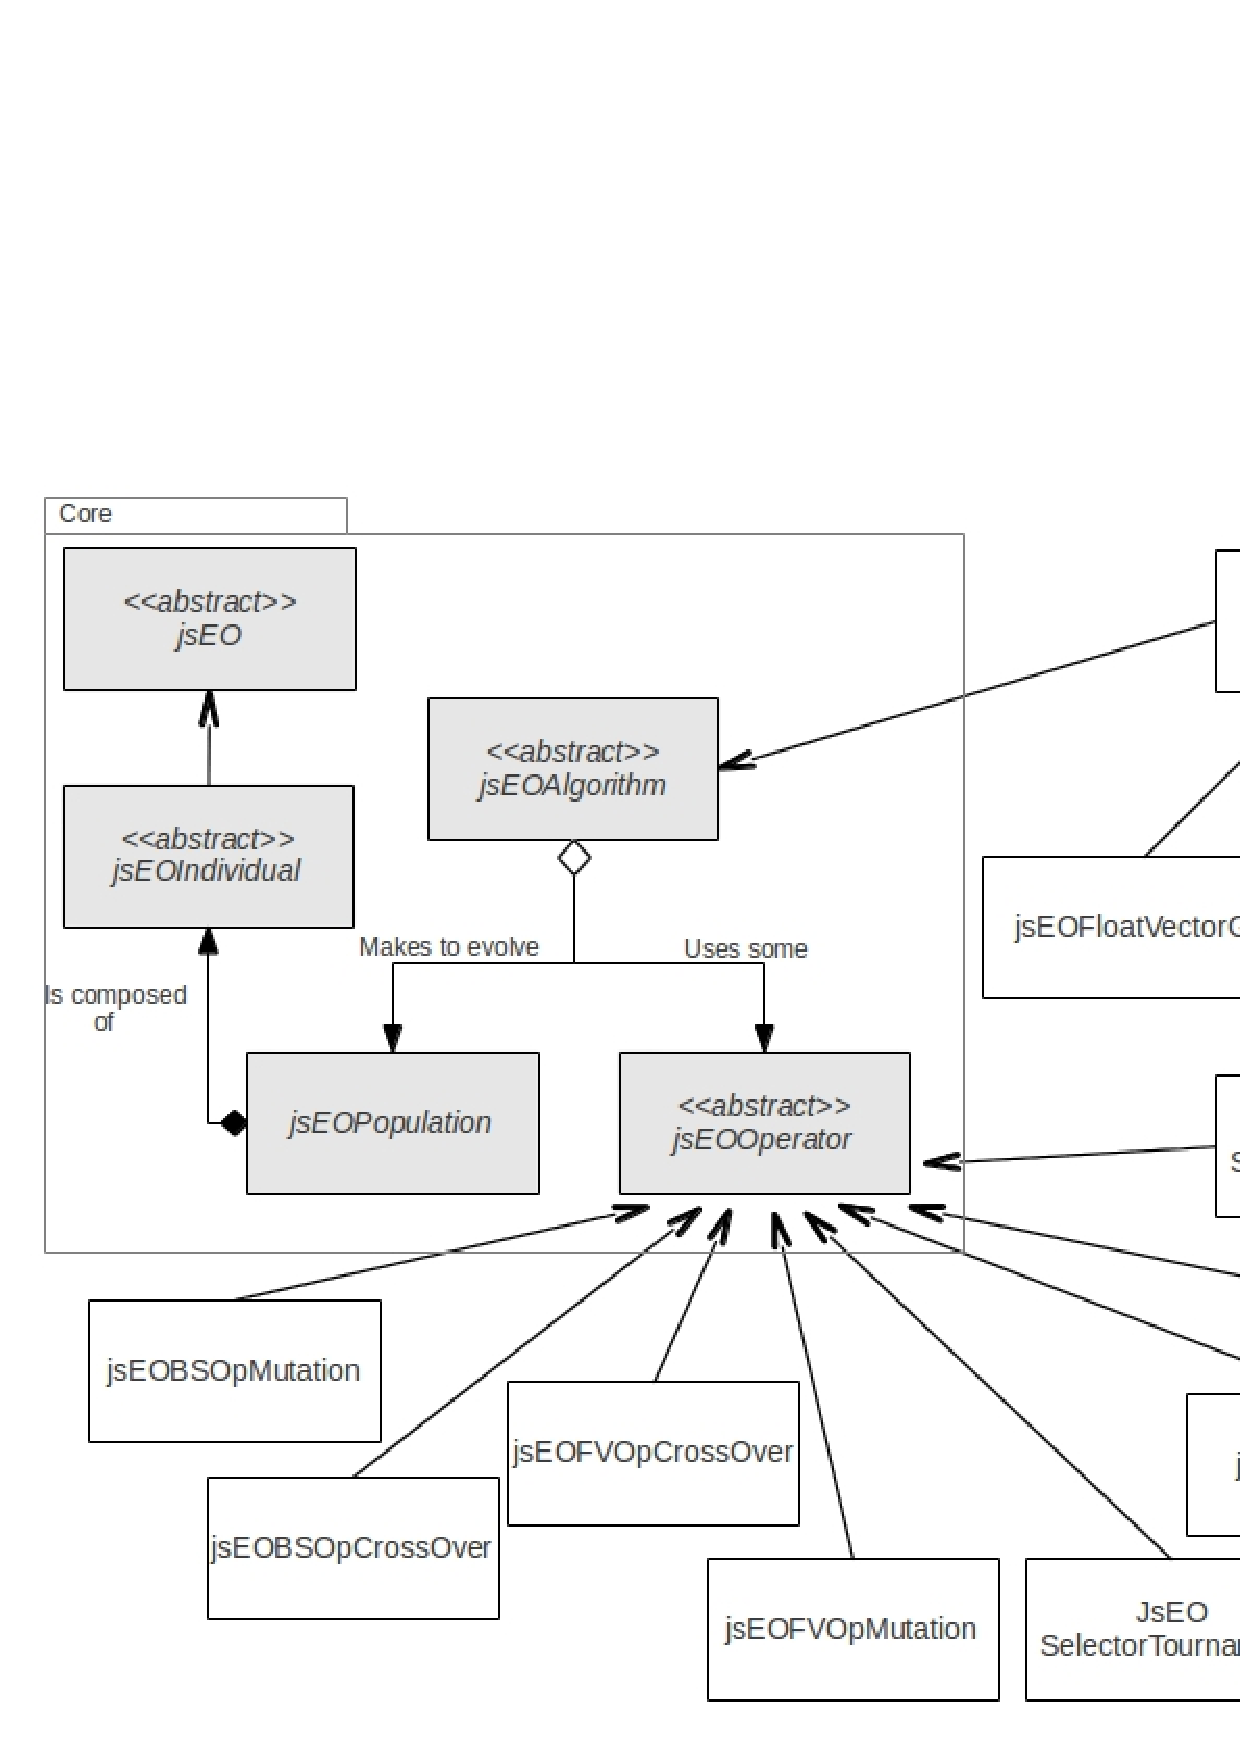
\includegraphics[height=10cm]{class-diagram.jpg}
\caption{One kernel at $x_s$ (\emph{dotted kernel}) or two kernels at
$x_i$ and $x_j$ (\textit{left and right}) lead to the same summed estimate
at $x_s$. This shows a figure consisting of different types of
lines. Elements of the figure described in the caption should be set in
italics, in parentheses, as shown in this sample caption.}
\label{fig:example}
\end{figure}

\section{Methodology and Experimental Setup}
\label{sec:method}
The experiments designed to the test jsEO include two problems, being the first the 256-bit Royal Road function, while the second is solving a 128-terms linear equation. In others words, the first one is related to a bit-string chromosome problem, while the second deals with vector of floats. Both problems have been executed as synchronized tasks, and are available at http://jseo.vrivas.es. Currently, synchronizing is quite constrained since it is done by means of AJAX connections to a server, whitout allowing to perform requests from pages hosted on a different one. 

Asking for collaboration to run the experiments was done publishing some messages in social nets as Facebook and Twitter, as well as sending an email to a group of about 70 computer-scientist professionals. From a potential target of more than 500 people, every experiment has been voluntarily executed ?? times (although many users did excute it more than once).

The user who wanted to participate in the experiments only had to
The algorithm runs on the client for a fixed number of generations
 running parameters are set from the server and are downloaded from
it along with the webpage from which the experiment is run. A preset
number of generations is run on the client, after with a request is
made to the server with the best individual in the last
generation. The algorithm stops and waits for the answer from the
server. The server receives the request, stores it in a database, and
sends back the best individual stored in the server. This individual
is incorporated in the client population, which starts again to run. 
Several clients acting at the same time make requests asynchronously,
using the facilities of the standard Apache web server. The server is
thus used as a clearinghouse for interchange of information among the
different clients; however, there's no explicit comunication or
topology among the different nodes running the genetic
algorithm. Besides, the fact that the server always contain the best
individuals generated so far guarantees that the best solution (with a
fixed number of evaluations resolution) available so far is always
kept. The server also sends back the number of generations the
client should run; which is usually the same number as before, but
turns to 0, thus stopping the client, when the stopping condition is
met. 

Clients leave the experiment by the expeditive method of surfing away
to another page or closing the web browser; in tabbed browsers (most
browsers nowadays), a tab (or several) can run the experiment while
the browser is available for other tasks. When the experiment has been
running for a predeterminad number of evaluations (which were set, for
this experiment, to 750000), all clients get a message to stop
running, and change their user interface to a message offering them to
reload the (new) experiment and start all over again. 
Besides, there is a {\em watching} daemon running on the server which
checks the database for the number of individuals evaluated, and
resets the experiment by incrementing the experiment ID by one and
eliminating the population. Thus, experiments can run unchecked on a
server while this {\sf watchgad} daemons is running. 
Several additional utilities are also provided via several webpages,
that inform on the state of the experiment, or allow to set the GA
parameters. 
Experimental subjects were gathered by several methods: sending it via
email to department and project coworkers, using the URL
for the experiment as a Google Plus or Facebook post, as a Twitter
(\url{http://twitter.com}) message, as a blog post,.

The experiment consisted in optimizing the  256-bits Royal Road
function, and each instance consisted in a maximum of 750000
evaluations (which were barely enough to find the solution). The
algorithm was steady state (with incorporation of the inmigrant every 20
generations), with rank-based selection and substitution; every
generation, 50\% of the population was generated, substituting the
worst 50\% individuals. Crossover priority was set to 80\%, and
mutation  to 20\%, changing 1\% of the bits. However, these settings
will have no influence on performance, other than the fact that, if
the solution is found before the end of the experiment, the users will
get bored and change to a new page\footnote{And this is just an example of how
social factors in this kind of experiments affect performance}.

Data was gathered from two different sources: the watcher-daemon logs,
which mainly gave data about the number of individuals evaluated and
the time needed for each experiment, and the Apache daemon log; the
relevant lines were extracted just by using {\sf grep}. It should be
noted that the server was not running exclusively the experiment, but
doing it along with the usual tasks. The server was a 700-MHz, 1
Gigabyte-RAM machine, with the database in another dual processor,
450-MHz machine. Both machines were running obsolete RedHat 7.x and
9.x Linux operating systems\footnote{Both machines host our group web
  server and home pages; we thought it was better to run the
  experiment in our standard setup instead of a dedicated
  setup}. 

Results of the experiment will be commented in the next section.

\section{Experimental results}
\label{sec:exp}


\section{Conclusions, discussion and future work}
\label{sec:conc}

While in previous papers  we proved that
this kind of AJAX based, volunteer, and potentially sneaky,
computation could be used profitably for performing genetic algorithm
experiments, in this paper we have proved that, 
without an expensive or far-fetched setup, it can achieve high
performance, equivalent, at most, to several computers of average
performance. The code used to perform the experiment is publicly
available and is modular so that creating different experiments is
just a matter of writing a new JavaScript fitness function and tuning
the GA parameters accordingly. 

The experiments have proved that there is a good amount of
computational power that can be easily tapped and used for
evolutionary computation experiments, however, the nature of jsEO
constrains also the way users donate computing power, as well as the
number of clients available for an experiment. In this paper we have
found some figures, which will undoubtedly vary for other experiments;
however, the general shape of the curves will probably be the same,
following a very steep decrease from the maximum values obtained. 

The GA, being asynchronous, faces some problems that have not been
tackled in this paper. What is the best approach to preserve
diversity? To generate a new population in each client, and receive
immigrants as soon as possible, which are incorporated into the
population? Or is it better to create new client populations based on
existing populations? What is really the algorithmic contribution of
new clients? These issues will be explored as future work. 
We will also try to measure the limits of this technology, and test
the impact of servers of varying performance and workload on overall
performance. Eventually, we will also try to perform a {\em sneaky}
experiment, to check what kind of performance can be expected in that
kind of setups. 



----
Enviado a JJ

Título:
Developing an object-oriented library in JavaScript to build modular and flexible cross-platform evolutionary algorithms 

Aims
Prove that it can be created a JavaScript library for evolutionary algorithms, that is object-oriented and, thus, modular and easily extensible.
Prove that this library can be used to execute evolutionary algorithms in web browsers. This allows to solve problems in the client side, but also to collaborate among many clients (if possible) to find better solutions by means of indidivuals migatrion using AJAX technology.

Methodology:
Consisted in
1) Creating the basic classes from which the rest will derivate: jsEO, jsEOIndividual, jsEOPopulation, jsEOOperator, jsEOAlgorithm
2) Derivating more specific classes, such as mutation and crossover operarators, as well as different kinds of individuals (e.g., bit-strings and float-strings).
3) Instantiating specifics objects to evaluate the library using the 256-royal road funcion, and a 128-terms equation.
4) Executing the experiments by means of simple web page access from many different devices (i.e., different microprocessors, operating systems, web browsers, amount of memory, or bandwidths among others).




De forma un poco más detallada:
1.1 Crear una biblioteca orientada a objetos con una clase básica: jsEO. Un objeto jsEO tiene asociado un fitness y, en base a dicho fitness, puede ser comparado con otro objeto jsEO.
1.2 A partir de dicho objeto derivar individuos (jsEOIndividual) que disponen de un cromosoma. Dicho cromosoma puede ser descodificado y evaluado obteniendo el correspondiente fitness.
1.3 Los individuos pueden ser agrupados en poblaciones (jsEOPopulation) las cuales pueden ser ordenadas por fitness.
1.4 Implementar la clase operador (jsEOOperator) que permita operar tanto sobre como poblaciones como sobre individuos
1.5. Finalmente, crear objetos algoritmos (jsEOAlgorithm) evolutivos los cuales puedan ser contener una población, un conjunto de operadores y una serie ordenada de instrucciones que permitan hacer evolucionar la población mediante la aplicación de los operadores.

2.1 Se definen un conjunto de operadores concretos, como el selector por torneo (jsEOTournament) o sobre individuos (como jsEOCrossOver). Dichos operadores permiten generar nuevas poblaciones a partir de las ya existentes realizando modificaciones en los individuos. 
2.2. Entre dichos operadores se ha definido uno que tansfiere un individuo de la población al servidor (jsEOSendIndividual), y otro que solicita al servidor que le envíe el individuo que tiene almacenado ((jsEOSendIndividual).

\section*{Acknowledgements}

Hidden for double-blind review

\bibliographystyle{unsrt}
\bibliography{evostar2007,GA-general,geneura,ror-js,volunteer}

% that's all folks
\end{document}
